\documentclass[12pt,a4paper]{article}
\usepackage{amsmath}
\usepackage[margin=2cm]{geometry}
\usepackage[english]{babel}
\usepackage[utf8]{inputenc}

\usepackage{setspace}
\usepackage{xcolor}

\usepackage{siunitx}
\sisetup{locale=DE}

\usepackage{booktabs}
\usepackage{graphicx}

\usepackage{float}
\usepackage{lmodern}
\usepackage[T1]{fontenc}

\begin{document}
\setlength{\parindent}{0pt}


\title{Computer Vision I - Sheet 2}
\author{Dominik Autaler, Jonas Otto (Group 2)}

\maketitle
\newpage

\section{Filter algebra}

\subsection{}
Given the filter $H = \left(\begin{array}{rrr}-1 & -2 & 0\\-2 & 0 & 2\\0 & 2 & 1\\\end{array}\right) $ and an Image I \in [0, 255] the exercise arises the question what minimum and maximum output values this filter could create. Because all values in the image are positive, the maximum of 1275 is reached for a pixel region like $\left(\begin{array}{rrr}0 & 0 & 0\\0 & 0 & 255\\0 & 255 & 255\\\end{array}\right) $. Analogous the minimim value of -1275 is for instance reached in a pixel region like $\left(\begin{array}{rrr}255 & 255 & 0\\255 & 0 & 0\\0 & 0 & 0\\\end{array}\right)$.

\subsection{}
The source code used for this exercise is located in sh02ex01.m. The resulting images for task 2 are shown in the figures 2 and 3. For comparison purposes the original image is displayed in figure 1. The filter H emphazises large constrasts along the diagonal from bottom left to the top right corner. Because the filter only emphazises high constrasts, it belongs to the class of high-pass filters.
 
\begin{figure}[h]
	\begin{center}
		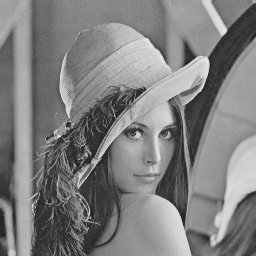
\includegraphics[scale=1]{./images/lena.png}
		\caption{Original image} 
	\end{center}
\end{figure}

\begin{figure}[h]
	\begin{center}
		
\includegraphics[scale=1]{./images/imG.png}
		\caption{Gaussian kernel applied to lena.tiff} 
	\end{center}
\end{figure}

\begin{figure}[h]
	\begin{center}
		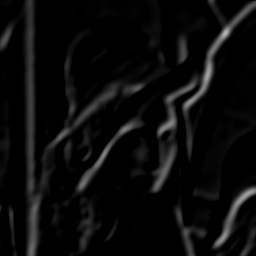
\includegraphics[scale=1]{./images/imR1}
		\caption{Resulting image for $R1 = I * G_{\sigma} * H$} 
	\end{center}
\end{figure}

\subsection{}
The figures 4 to 6 show the results to task 3. Although the image shown in figure 6 looks quite dark, the sum over all pixels in the image is aproximately 31. Compared to the size of the image (256px x 256px) this number is so small, the one could argue that the error is coming from the small inaccuraries related to calculating with floating point numbers. 
Therefore the example shows the commutative property the convolution owns quite well. 

\begin{figure}[h]
	\begin{center}
		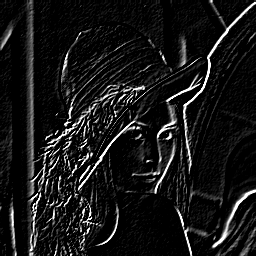
\includegraphics[scale=1]{./images/imH.png}
		\caption{Filter H applied to lena.tiff} 
	\end{center}
\end{figure}

\begin{figure}[h]
	\begin{center}
		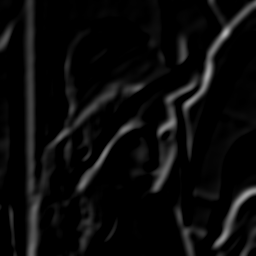
\includegraphics[scale=1]{./images/imR2.png}
		\caption{Resulting image for $R2 = I * H * G_{\sigma}$} 
	\end{center}
\end{figure}

\begin{figure}[h]
	\begin{center}
		
\includegraphics[scale=1]{./images/imDiff.png}
		\caption{Resulting image for |R1 - R2|} 
	\end{center}
\end{figure}

\clearpage
\section{Discrete Fourier Transform}
\subsection{}
Our implementation of the Discrete Fourier Transform can be found in the file fourier.m. Figure 7 shows the results of applying our DFT to the given signal.

\begin{figure}[h]
	\begin{center}
		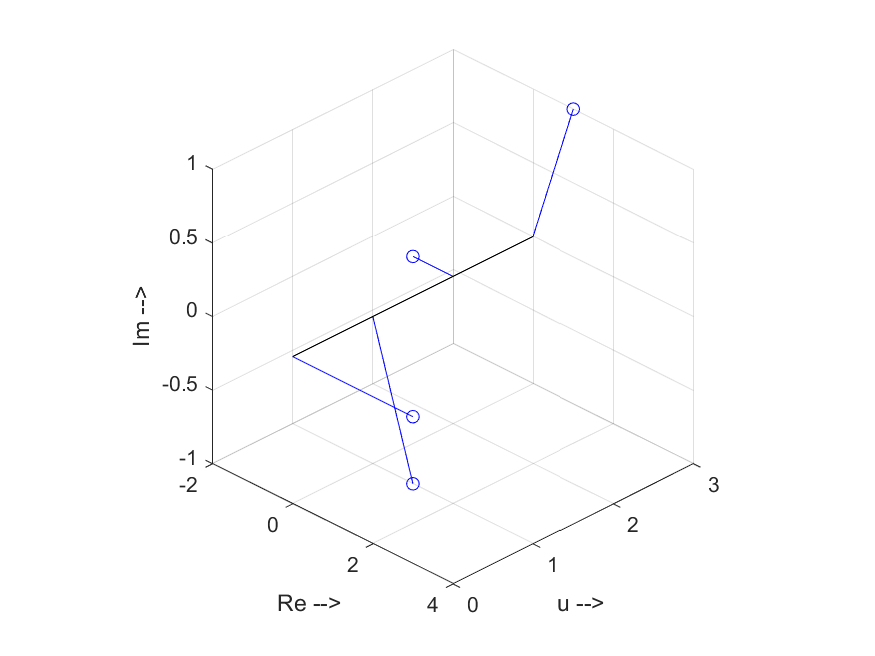
\includegraphics[scale=1]{./images/Stemcomplex.png}
		\caption{Complex visualization of the results of the DFT} 
	\end{center}
\end{figure}

\subsection{}
Figure 8 shows the sine wave which corresponds to the vector at u = 1 in Figure 7. Because this vector has both a real and an imaginary component not equal to zero it would also create a cosine wave. Both waves together would then represent this part in the original signal.
\begin{figure}[h]
	\begin{center}
		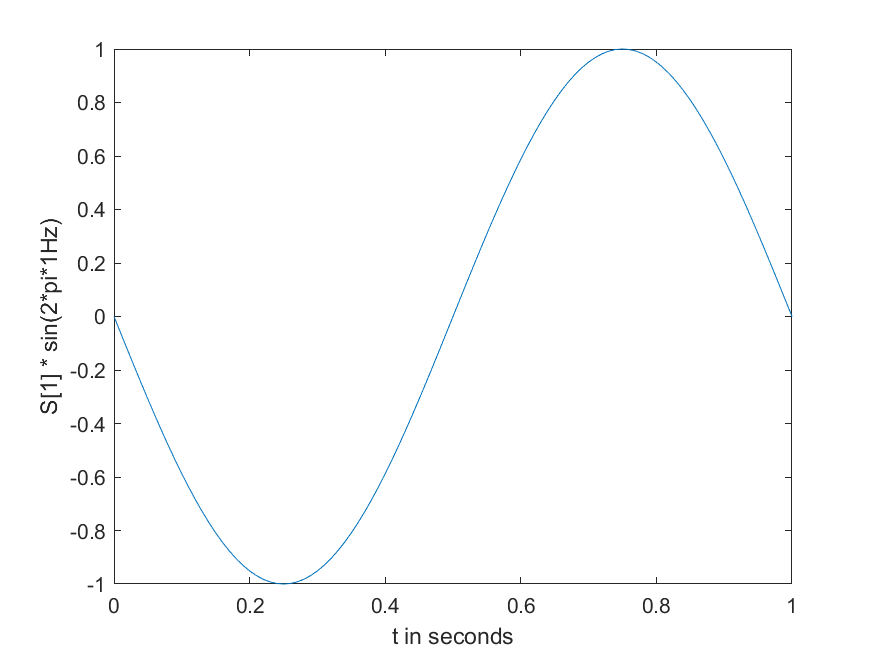
\includegraphics[scale=1.0]{./images/Sinus.png}
		\caption{Sinus component of the complex value representing 1Hz} 
	\end{center}
\end{figure}

\subsection{}
The source code used for this task can be found in the file ifourier.m.

\subsection{}
Figure 9 shows the results gained from task a) to c). Because the third value of the reconstructed signal is not exact zero but of the magnitude $10^{-16}$ Matlab expands the vertical axis in the third plot a bit into the negative direction. Besides this small difference, the reconstructed signal looks the same compared to the orignal signal. Because our signal was sampled with a sampling frequency of 4$\si{Hz}$ and the sampled signal has 4 points, the frequency resolution of the frequency spectrum is $\frac{4\si{Hz}}{4} = 1\si{Hz}$.

\begin{figure}[h]
	\begin{center}
		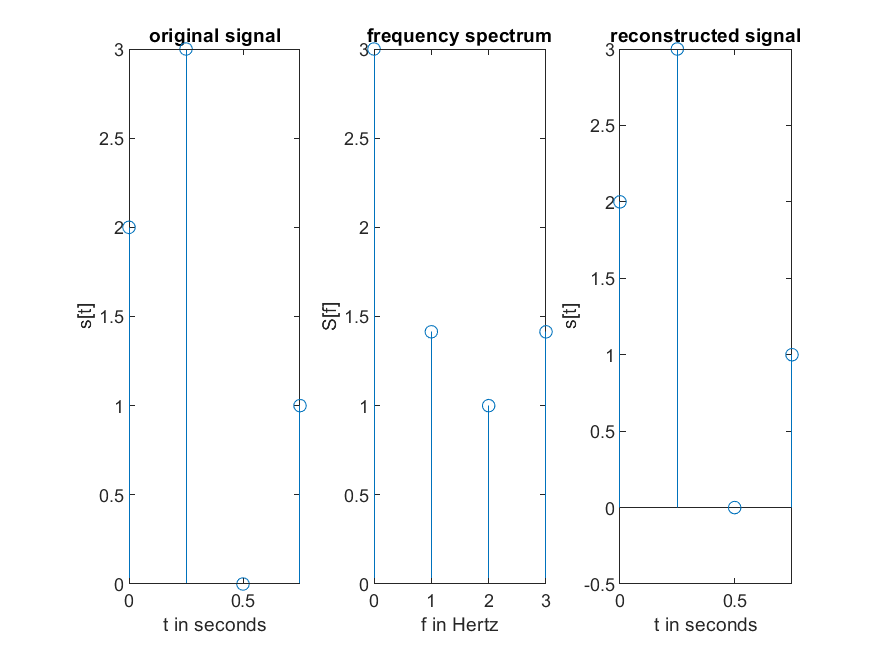
\includegraphics[scale=1.0]{./images/figure_d.png}
		\caption{Plots showing results from task a) to c)} 
	\end{center}
\end{figure}

\clearpage
\section{Fourier Transform for Image Quality Assessment}
The source used to create the figures shown in this section can be found in the Matlab script sh03ex03.m.
Figure 10 shows the original images together with their frequency spectra calculated with fft2. The spectra have been shifted by using fftshift. Moreover they are showing the absolute values with an logarithmic scale. Figure 11 showes the highpass filter which was used in the next tasks.

\begin{figure}[h]
	\begin{center}
		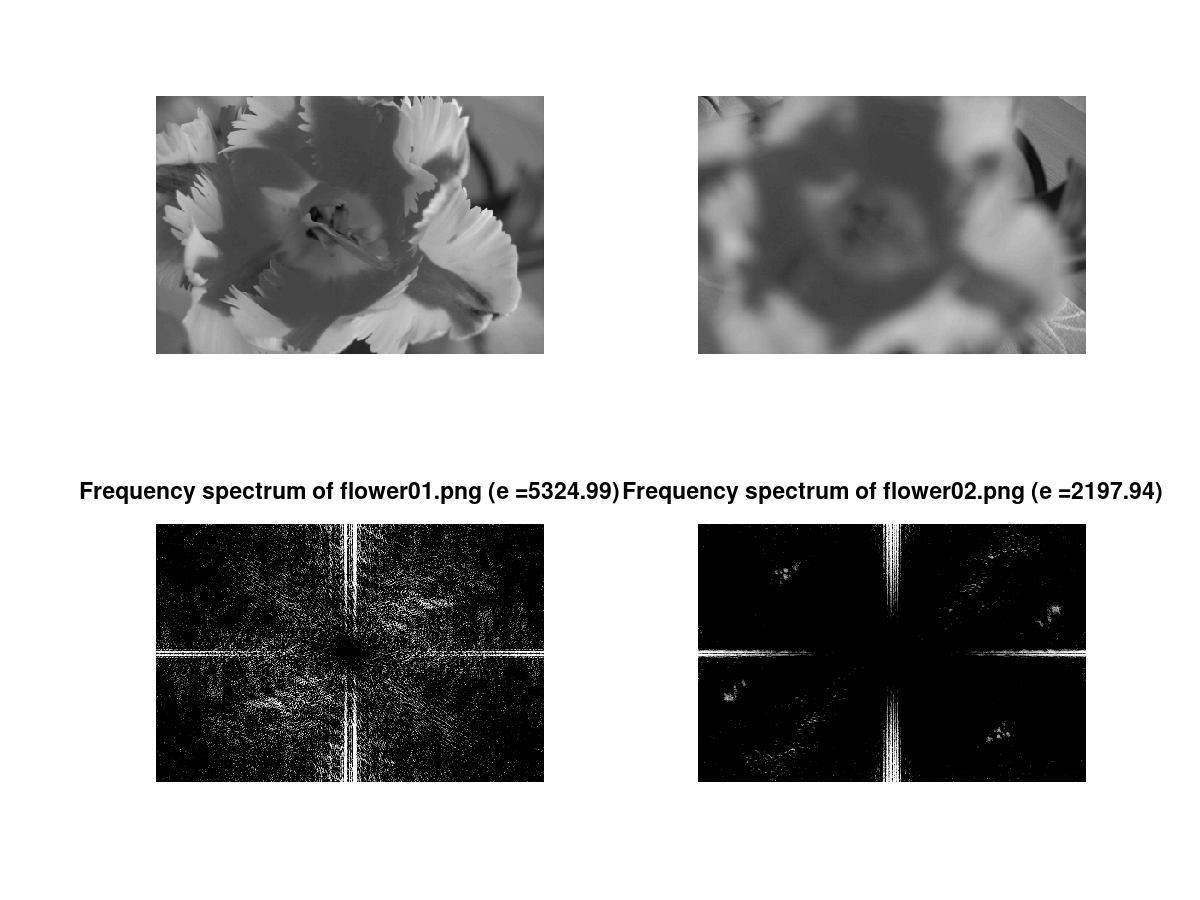
\includegraphics[scale=1.0]{./images/ex03_1.png}
		\caption{Original images and their frequency spectra} 
	\end{center}
\end{figure}

\begin{figure}[h]
	\begin{center}
		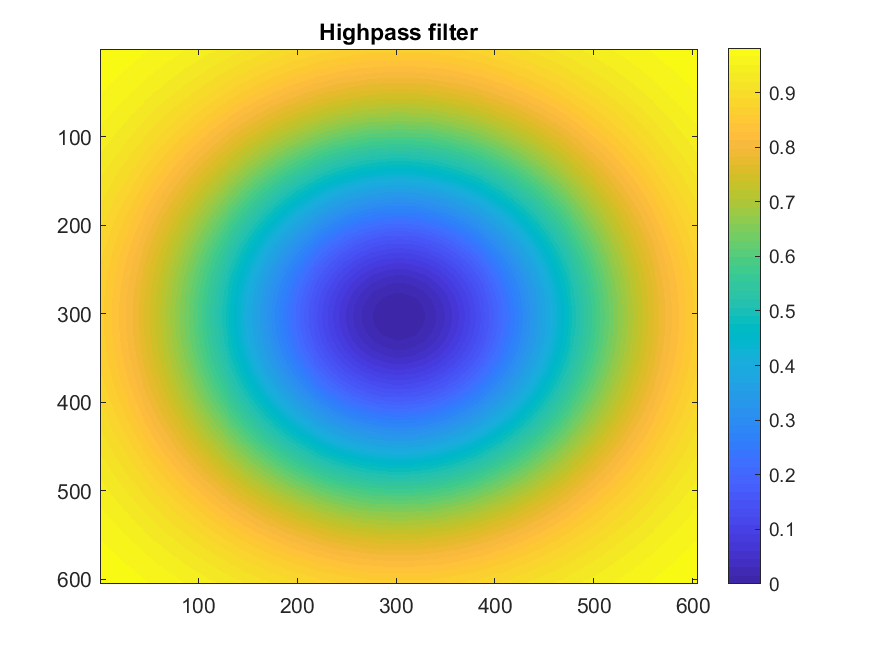
\includegraphics[scale=1.0]{./images/ex03_2.png}
		\caption{Highpass filter} 
	\end{center}
\end{figure}

\end{document}